% Chapter 4

\chapter{Methodology} % Main chapter title

\label{Chapter4} % For referencing the chapter elsewhere, use \ref{Chapter4} 

In this chapter we present the methodology of the research. First we present the threat model. After that, we show the overview of the implementation of the ScaRR algorithm to extract checkpoint and list of action. The section about ScaRR control-flow model will follow. The last two section is the detail on LLVM implementation to get checkpoints and list of actions from codes. Checkpoints and list of actions are collected to build offline measurement database that is used for the remote attestation.

\section{Threat Model}

The threat model in this research from ScaRR threat model \cite{toffaliniScaRRScalableRuntime2019}. There are two parties: attacker and prover. The attacker has aim to hijact the application control flow by using various memory attacks described in Chapter \ref{Chapter3}. However, we do not consider physical attack and data-oriented attack which does not alter program CFG. The prover uses kernel as trusted anchor and has common memory corruption attack mitigations such as \( W \bigoplus R \) and ASLR. 

\section{Overview of The Offline Measurement}

The goal of the offline measurement is to get the information to be used in the remote attestation. In this research we implement ScaRR Control-flow model \cite{toffaliniScaRRScalableRuntime2019} which we also elaborate in the Section \ref{sec:scarr-model}. These are the steps that we do in getting the offline measurements:

\begin{enumerate}
    \item Flattenning the CFG
    \item Marking the Checkpoints
    \item Finding the List of Actions
\end{enumerate}

\begin{listing}[htbp]
    \begin{minted}[
        frame=lines,
        framesep=2mm,
        baselinestretch=1.2,
        fontsize=\footnotesize
        ]{c++}
        int main() {
            for (int i = 0; i < 10; i++) {
                // do nothing
            }
        }
    \end{minted}
    \caption{Simple Loop}    
    \label{listing:simple-loop}
\end{listing}

\subsection{Flattenning the CFG}

Consider the program in listing \ref{listing:simple-loop}. The CFG is shown in the figure \ref{fig:simple-loop-cfg}. The first step of the offline measurement is to flatten the CFG to get all the basic block list. We can flatten the CFG into basic block with one out of some graph traversal algorithm in LLVM. The CFG in figure \ref{fig:simple-loop-cfg} contains these following basic blocks:

\begin{itemize}
    \item Basic Block \%0
    \item Basic Block \%3
    \item Basic Block \%6
    \item Basic Block \%7
    \item Basic Block \%10
\end{itemize}


\begin{figure}[htbp]
\centerline{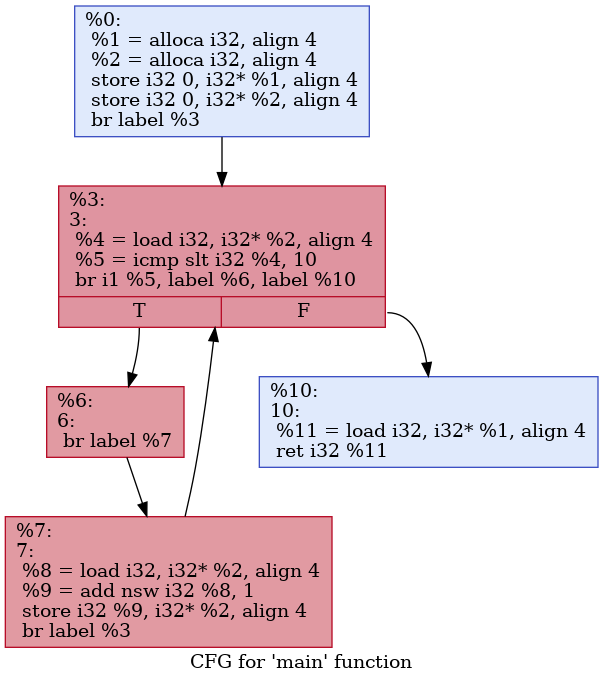
\includegraphics[scale=.5]{Figures/04/simple-loop.png}}
\caption{Simple Loop CFG}
\label{fig:simple-loop-cfg}
\end{figure}

\subsection{Marking the Checkpoints}


After we flatten CFG into basic block, we will check each of basic block to find different kind of checkpoints. The marked checkpoints from the CFG in Figure \ref{fig:simple-loop-cfg} can be seen in Figure \ref{fig:simple-loop-checkpoints}.

\begin{figure}[htbp]
\centerline{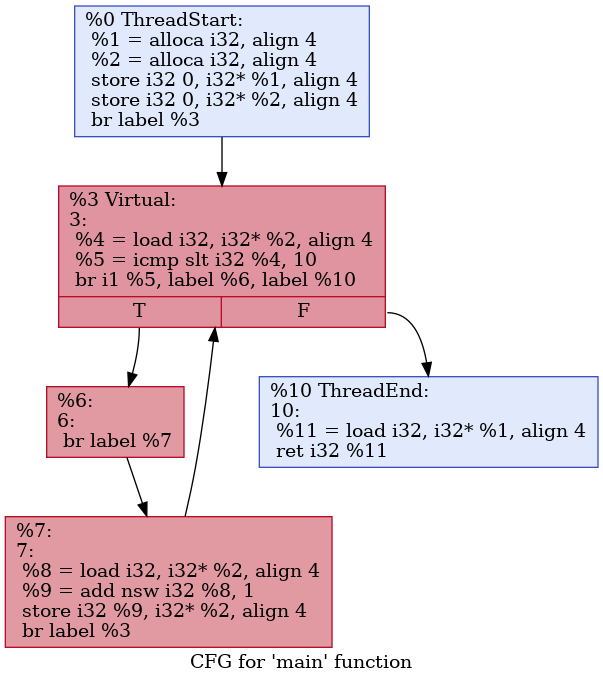
\includegraphics[scale=.5]{Figures/04/simple-loop-checkpoints.png}}
\caption{Loop CFG}
\label{fig:simple-loop-checkpoints}
\end{figure}

\subsection{Finding the List of Actions}

The step of finding LoA is traversing path between two checkpoints and add significant basic block that traverse the path between the two checkpoints. The detail of this step is explained in the next sections.

\section{ScaRR Control-Flow Model} \label{sec:scarr-model}

ScaRR \cite{toffaliniScaRRScalableRuntime2019} are taking lesson learned from many former runtime remote attestation scheme to build model that can perform in a scalable way and can perform remote attestation on complex system. ScaRR control-flow model consists of two main components, checkpoint and list of action. 

As many previous runtime attestation scheme, ScaRR models and validates the attestion based on program's control flow graph. We need to run one-time measurement computation to extract checkpoints and list of actions of the program.

\subsection{Checkpoints} \label{sec:scarr-checkpoints}
Checkpoint is basic block of the program that delimit execution path of the program. ScaRR defines these different checkpoint types:
\begin{itemize}
    \item Thread Beginning: demarcating the start of program/thread
    \item Thread End: demarcating the end of program/thread
    \item Exit Point: representing exit point from application such as system call or out of translation unit function/library call
    \item Virtual-Checkpoint: managing cases for loop or recursion
\end{itemize}

In a program there should be at least Thread Beginning and Thread End checkpoints. Later depends on the structure of the program different checkpoint is marked in the program CFG.

\subsection{List of Actions}

List of actions (LoA) are edges (marked by two checkpoints) that direct one checkpoint to the next one. In program execution path, we only consider edges that identify the unique execution path.

LoA is defined through the following notation:

$$[(BBL_{s1},BBL_{d1}),...,(BBL_{sn},BBL_{dn})]$$

Consider again the CFG in the Figure \ref{fig:simple-loop-checkpoints}. The LoA between node 3 (Checkpoint Virtual) and node 10 (checkpoint ThreadEnd) is  $[(BBL_3, BBL_{10})]$. However, the LoA between node 0 and node 3 is $[]$ (empty set).

\section{ScaRR LLVM Pass} 

ScaRR LLVM pass\footnote{https://github.com/lamida/llvm-project/pull/3} is the implementation of ScaRR offline measurement using LLVM. ScaRR offline measurement is represented as the following key-value pair.

$$(cp_A, cp_B, H(LoA)) \Rightarrow [(BBL_{s1}, BBL_{d1}), ..., (BBL_{sn}, BBL_{dn})]$$

As described in the section \ref{sec:scarr-checkpoints}, checkpoint is a special basic block that delimit path between execution path in a CFG. $cp_A$ is the start delimiter of the path. $cp_B$ is the end of delimiter. $LoA$ — list of action — is list of significant basic block pairs which define edges 

ScaRR extractor traverses the graph in two passes. The first pass is find whether the basic block is a checkpoint (section \ref{sec:scarr-checkpoint-marker}). The second pass traverses the graph and mark List of Action between every two checkpoint (section \ref{sec:scarr-loa-collector}). 

\section{ScaRR Checkpoint Marker} \label{sec:scarr-checkpoint-marker}

The logic of checkpoint marker is to traverse the whole control flow graph at least once. For each basic block, we have to check whether the basic block can be considered as any of checkpoint type mentioned above. To allow marking additional information about ScaRR checkpoint, we are modifying the BasicBlock class to add checkpoint instance variable as shown in listing \ref{listing:checkpoint}.

\begin{listing}[htbp]
    \begin{minted}[
        frame=lines,
        framesep=2mm,
        baselinestretch=1.2,
        fontsize=\footnotesize,
        linenos
    ]{c++}
        class BasicBlock ... {
        private:
        // add checkpoint field
            Checkpoint cp;

        public:
            // setter and accessor
        void setCheckpoint(Checkpoint);
        Checkpoint getCheckpoint() const;
        ...
        }
    \end{minted}
    \caption{Add Checkpoint Instance Variable to BasicBlock class.}    
    \label{listing:checkpoint}
\end{listing}

The algorithm to mark the checkpoint is first we iterate all basic block in main function. First we mark the first basic block with no predecessor as ThreadStart checkpoint and basic block with no successor and ThreadEnd checkpoint. 

To identify ExitPoint checkpoint, for each basic block then we iterate  each instruction to find whether any instruction in the basic block is a `call` instruction and has no body defined in this translation unit. Please refer to Listing \ref{listing:exit-point-cp}.

\begin{listing}[htbp]
    \begin{minted}[
        frame=lines,
        framesep=2mm,
        baselinestretch=1.2,
        fontsize=\footnotesize,
        linenos
    ]{c++}
        for (auto &basicBlock: Function) {
            for (auto &instruction : basicBlock) {
                if (isa<CallInst>(i)) {
                auto *call = &cast<CallBase>(i);
                if (call != nullptr && call->getCalledFunction()->empty()) {
                    // this basicBlock is ExitPoint
                    basicBlock.setCheckpoint(Checkpoint::ExitPoint);
                } 
            }
        } 
    \end{minted}
    \caption{Finding ExitPoint Checkpoint}    
    \label{listing:exit-point-cp}
\end{listing}

To mark Virtual checkpoint, we need to find loop header basic block. Although there is no direct API to check whether a basic block is a loop header, LLVM provide it in LoopInfoBase API. See Listing \ref{listing:virtual-cp}

\begin{listing}[htbp]
    \begin{minted}[
        frame=lines,
        framesep=2mm,
        baselinestretch=1.2,
        fontsize=\footnotesize,
        linenos
    ]{c++}
        void findVirtualCheckpoint(DominatorTree &DT, Function &F) {
            DT.recalculate(F);
            // generate the LoopInfoBase for the current function
            LoopInfoBase<BasicBlock, Loop>* KLoop = new LoopInfoBase<BasicBlock, Loop>();
            KLoop->releaseMemory();
            KLoop->analyze(DT);
            for (auto &bb : F) {
                // Since the BasicBlock would have been inlined, just traverse from main function
                if (F.getName() == "main") {
                auto loop = KLoop->getLoopFor(&bb);
                if (loop != nullptr) {
                    // found VirtualCheckpoint
                            loop->getHeader()->setCheckpoint(Checkpoint::Virtual);
                }
                }
            }
        }
    \end{minted}
    \caption{Getting Virtual Checkpoint}
    \label{listing:virtual-cp}
\end{listing}

\section{ScaRR LoA Collector} \label{sec:scarr-loa-collector}

The algorithm of getting LoA between two checkpoints is little bit more complex. First, we iterate all the basic block and if the basic block is a checkpoint we mark this is $cpA$. Next, we recursively traverse the successor of $cpA$ until we find another checkpoint $cpB$. It is possible for $cpA = cpB$. If there is no branch between the two checkpoint, the LoA is an empty set. If there is a branch, the first LoA is always be $cpA$ and the second LoA is always be the first basic block after the branch \textemdash{} which can be $cpB$ or just non checkpoint basic block. Interested readers can refer to the implementation of this pass to see the detail.

\subsection{Running The Pass}

To mark the list of Checkpoints, we can invoke LLVM \texttt{opt} as shown in listing \ref{listing:mark-cp-in-cfg}.

\begin{listing}[htbp]
    \begin{minted}[
        frame=lines,
        framesep=2mm,
        baselinestretch=1.2,
        fontsize=\footnotesize,
    ]{c++}
        opt -passes=scarr-cp-marker <file>.ll
    \end{minted}
    \caption{Mark Checkpoint in BasicBlock}    
    \label{listing:mark-cp-in-cfg}
\end{listing}

We can see the basic blocks output that has been marked with checkpoint using LLVM dot-cfg pass.

\begin{listing}[htbp]
    \begin{minted}[
        frame=lines,
        framesep=2mm,
        baselinestretch=1.2,
        fontsize=\footnotesize,
    ]{c++}
        opt -passes=scarr-cp-marker,dot-cfg <file>.ll
    \end{minted}
    \caption{Print Checkpoints in CFG dot file}    
    \label{listing:cp-to-cfg}
\end{listing}

The commands in listing \ref{listing:cp-to-cfg} generates different dot files per function. We can use xdot command line from graphiz to see the graph. 

To mark the list of actions between checkpoints, we can invoke LLVM \texttt{opt} as shown in Listing \ref{listing:get-loa}

\begin{listing}
    \begin{minted}[
        frame=lines,
        framesep=2mm,
        baselinestretch=1.2,
        fontsize=\footnotesize,
    ]{c++}
        opt -passes=scarr-cp-marker,scarr-loa-collector <file>.ll
    \end{minted}
    \caption{Get List of Actions}    
    \label{listing:get-loa}
\end{listing}

Note that we have to run scarr-cp-marker before scarr-loa-collector.

The result and its interpretation are discussed in the next chapter.